\documentclass[tikz,border=10pt]{standalone}
\usepackage{amsmath,amssymb}
\usepackage{tikz}
\usetikzlibrary{arrows,automata,backgrounds,calendar,chains,decorations,decorations.pathreplacing,decorations.text,fit,matrix,mindmap,patterns,petri,plotmarks,positioning,shadows,shapes,shapes.callouts,shapes.geometric,shapes.misc,spy,trees,calc,intersections,tikzmark,arrows.meta}
\usepackage{xcolor}
\usepackage{pgfplots}
\pgfplotsset{compat=1.16}

% Common math macros from the book
\def\x{\mathbf{x}}
\def\y{\mathbf{y}}
\def\z{\mathbf{z}}
\def\A{\mathbf{A}}
\def\b{\mathbf{b}}
\def\c{\mathbf{c}}
\def\w{\mathbf{w}}
\def\v{\mathbf{v}}
\def\u{\mathbf{u}}
\def\e{\mathbf{e}}
\def\zero{\mathbf{0}}
\def\R{\mathbb{R}}
\def\N{\mathbb{N}}
\def\Z{\mathbb{Z}}
\def\Q{\mathbb{Q}}
\def\st{\text{s.t.}}
\def\vect#1{\mathbf{#1}}
\def\xLP{x^{\mathrm{LP}}}
\def\zLP{z^{\mathrm{LP}}}
\def\xIP{x^{\mathrm{IP}}}

% Common node styles from the book
\tikzset{
    main/.style={circle, draw, fill=gray!20, minimum size=1cm, font=\normalsize},
    dot/.style={circle,fill=blue,minimum size=3pt,inner sep=0pt, outer sep=-1pt},
    vertex/.style={circle,fill=black!25,minimum size=20pt,inner sep=0pt},
    edge/.style={draw,-,thick},
    directed edge/.style={draw,->,>=latex,thick},
}

% Additional macros for 3D/coordinate systems
\newcommand{\xhat}{\hat{\x}}
\newcommand{\yhat}{\hat{\y}}
\newcommand{\zhat}{\hat{\z}}
\newcommand{\ihat}{\hat{\imath}}
\newcommand{\jhat}{\hat{\jmath}}
\newcommand{\khat}{\hat{k}}

\begin{document}
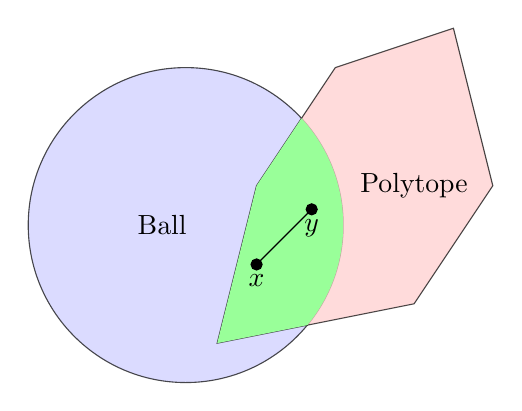
\begin{tikzpicture}

% Draw the circle (ball in 2D) slightly to the left
\filldraw[blue!20, opacity=0.7, draw = black] (0.1,1.5) circle (2cm);

% Draw the 6-vertex polytope slightly to the right
\filldraw[red!20, opacity=0.7, draw = black] (0.5,0) -- (3,0.5) -- (4,2) -- (3.5,4) -- (2,3.5) -- (1,2) -- cycle;

% Shade the intersection
\begin{scope}
  \clip (0.1,1.5) circle (2cm);
  \fill[green!40] (0.5,0) -- (3,0.5) -- (4,2) -- (3.5,4) -- (2,3.5) -- (1,2) -- cycle;
\end{scope}

% Label the circle and polytope
\node at (-0.2,1.5) {Ball};
\node at (3,2) {Polytope};

% Define the points
\coordinate (x) at (1,1);
\coordinate (y) at (1.7,1.7);
\coordinate (z) at (2/3*1 + 1/3*1.7, 2/3*1 + 1/3*1.7);

% Plot the line segment between x and y
\draw (x) -- (y);

% Mark the points with dots and labels
\filldraw [black] (x) circle (2pt) node[anchor=north] {$x$};
\filldraw [black] (y) circle (2pt) node[anchor=north] {$y$};
%\filldraw [red] (z) circle (2pt) node[anchor=south east] {};%$z = \lambda x + (1-\lambda)y$};
\end{tikzpicture}
\end{document}
